		
		\section{NAIVER ANSATZ ALT} \label{sec:ueberblick} 

		\todo{chap: Lsgansatz section: Naiver Ansatz --> Mergen nach Lösungsansatz Einführung} 

		Enthält ein Datensatz Informationen zu einem geografischen Objekt, so können in diesem geografische Indikatoren enthalten sein.
		Durch diese geografischen Indikatoren kann dem Datensatz, und damit dem geografischen Objekt, eine Georeferenz zugewiesen werden. 

		Die Zuordnung einer Georeferenz mit Hilfe von geografischen Indikatoren soll Geolokalisierung genannt werden.  

		In Abbildung \ref{img:geolokalisierung} wird dies dargestellt.
		Im Gegensatz zu Abbildung \ref{img:geogIndi} ist kein direkter Verweis vom geografischen Objekt zu einer Georeferenz vorhanden. 
		Stattdessen wird mit Hilfe der geografischen Indikatoren a und b durch die Geolokalisierung eine Georeferenz zugeordnet.

		\begin{figure}[!ht]
		\begin{center}
		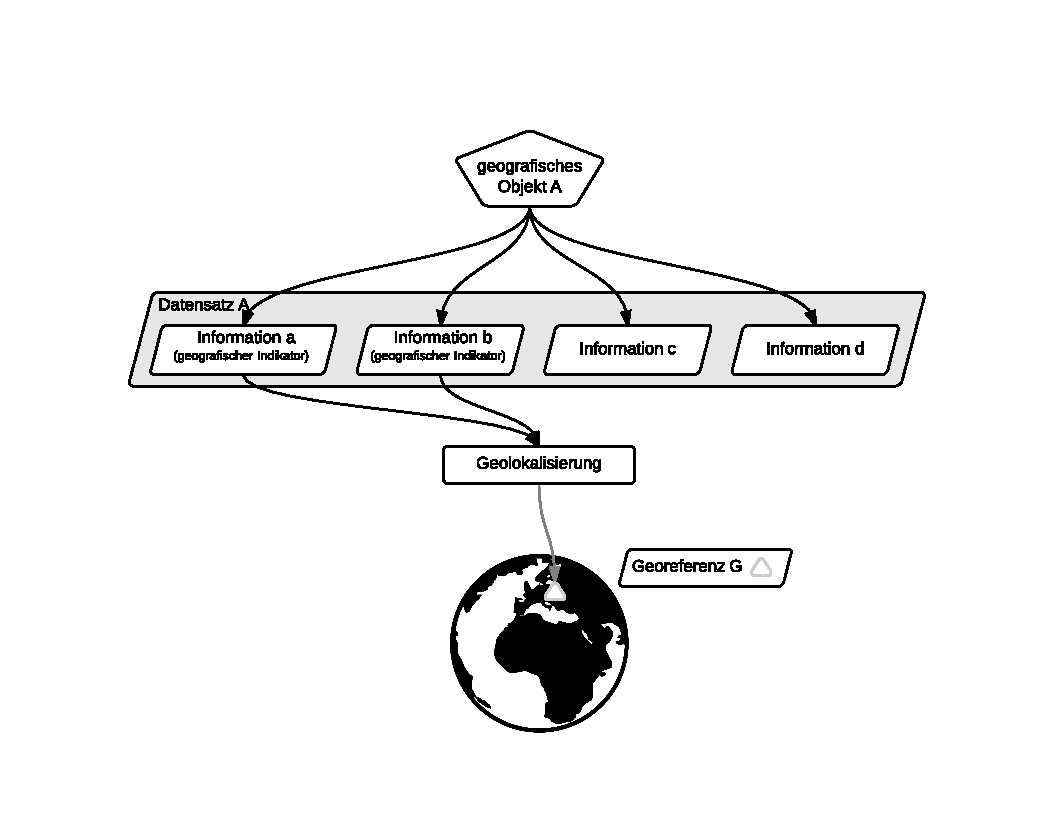
\includegraphics[scale=1.0]{geolokalisierung.pdf}
		\caption{Geografische Hierarchieebenen}
		\label{img:geolokalisierung}
		\end{center}
		\end{figure}	

		Um aus den geografischen Indikatoren eine Georeferenz ableiten zu können soll eine Datenbasis verwendet werden.
		Diese ordnet den geografischen Indikatoren eine Georeferenz zu.
		Die gespeicherte Georeferenz ist bekannt und kann genau bestimmt werden. 
		Das bedeutet: Ein Hinweis auf eine geografische Position wird auf eine konkrete, bekannte geografische Position abgebildet.
		Eine solche Datenbasis soll Georeferenz-Basis genannt werden.  

		Im einfachsten Fall liegt ein geografischer Indikator vor, dem direkt eine Georeferenz zugewiesen werden kann.
		Dies kann Beispielsweise ein eindeutiges Toponym sein.	
		Ein Ortsverzeichnis könnte hier als Georeferenz-Basis verwendet werden.
		Liegt der Datenwert "'Karlsruhe"' vor so würde die Geolokalisierung durch eine Abfrage an die Georeferenz-Basis die Stadt Karlsruhe als Georeferenz zuweisen.

		Wie in Kapitel \ref{sec:ToponymeInGeografischenIndikatoren} bereits erläutert sind Toponyme allerdings nicht immer eindeutig oder bekannt. 
		Die Abfrage an ein Ortsverzeichnis liefert potenziell mehrere Ergebnisse was eine weitere Verarbeitung der Ergebnisse erfordert.
		Ist das Toponym nicht bekannt so kann kein Ergebnis geliefert.

		Des weiteren sind die Datenwerte eines Datensatzes nicht immer direkt zu verwenden.
		Dies kommt ganz darauf an wie die Daten erhoben wurden. 
		Nutzereingaben auf Webseiten können beispielsweise aus einer Liste gewählt, oder in ein Freitext-Feld eingegeben werden.
		Werden die Datenwerte durch eine Liste erhoben liegt eine klar definierte Menge an möglichen Datenwerten vor.
		Haben die Datenwerte in der Liste geografischen Bezug so können ihnen Georeferenzen zugeordnet werden.
		Die so entstandenen Paare aus Datenwert und Georeferenz können in der Georeferenz-Basis abgespeichert werden.

		Soll ein Nutzer in ein Freitext-Feld seinen aktuellen Standort eingeben, und der Datenwert wird direkt übernommen muss dieser vorverarbeitet werden.
		Es ist zwar wahrscheinlich, dass der Nutzer ein Toponym angibt, aber es kann durch die direkte Übernahme der Eingabe zu Problemen kommen.
		Zunächst kann nicht einmal entschieden werden ob der Datenwert überhaupt einen geografischen Indikator darstellt.
		Zudem können in einem Freitext-Feld mehrere geografische Indikatoren auftauchen.
		Diese können widersprüchlich sein oder aber eine geografische Position genauer spezifizieren. 
		Durch die direkte Übernahme des Wertes können alle in Kapitel \ref{sec:ToponymeInGeografischenIndikatoren} aufgeführten Probleme auftreten.
		Dies macht die Zuordnung einer Georeferenz durch eine Ortsverzeichnis schwierig.
		Soll trotzdem mit Hilfe eines Ortsverzeichnisses eine Geolokalisierung durchgeführt werden ist zumindest eine umfangreiche Vor- und Nachverarbeitung nötig.

		In Abbildung \ref{img:geolokalisierungBsp} ist ein Beispiel zur Verwendung einer Georeferenz-Basis dargestellt.
		Der Datenwert "'Karlsruhe"' wird dabei auf eine Georeferenz aufgelöst indem eine Abfrage an die Georeferenz-Basis durchgeführt wird.
		Die zurückgelieferte Georeferenz wird dem Datensatz zugeordnet.

		\begin{figure}[!ht]
		\begin{center}
		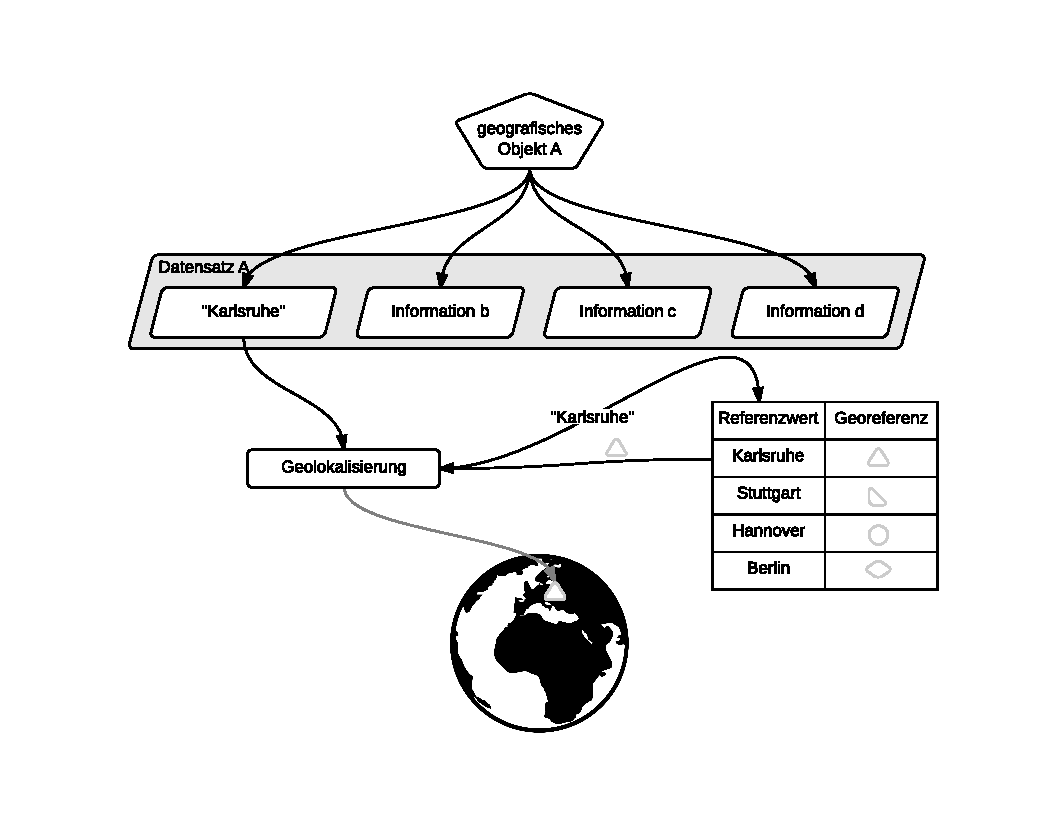
\includegraphics[scale=1.0]{geolokalisierungBsp.pdf}
		\caption{Geolokalisierung mit Referenz-Basis}
		\label{img:geolokalisierungBsp}
		\end{center}
		\end{figure}	

		Im folgenden Kapitel soll eine erste Struktur für eine Georeferenz-Basis vorgestellt werden.
		Es sollen dabei die minimalen Anforderungen an eine solche Datenbasis erfüllt werden.

	\section{MINIMALE STRUKTUR GEOREFERENZ BASIS ALT} \label{sec:generelleStruktur} 
		
		\todo{chap: Lösungsansatz sec: minimale Struktur Georef Basis alr ----> Schauen ob obsolet oder Mergen nach } 

		Nach Abbildung \ref{img:geolokalisierung} wird bei der Geolokalisierung einem oder mehreren geografischen Indikatoren eine Georeferenz zugewiesen.
		In der einfachsten Variante wird lediglich ein einziger geografischer Indikator an die Geolokalisierung übergeben, und genau eine Georeferenz zurückgegeben.
		Die Geolokalisierung muss also zu einem gegebenen geografischen Indikator eine Georeferenz bestimmen können.
		Dies führt zu einer ersten einfachen Struktur für die Georeferenz-Basis.	

		Es wird angenommen der geografische Indikator stellt immer ein eindeutiges Toponym dar.
		Des weiteren sind alle möglichen Toponyme sowie eine zugehörige Georeferenz bekannt. 
		Die Georeferenz liegt als Adresse mit Straße, Hausnummer, Postleitzahl und Ortsname vor.

		Jedem möglichen Toponym soll eine Georeferenz zugeordnet werden können. 
		Die Georeferenz-Basis muss also eine Menge von Toponymen und zugehörigen Georeferenzen beinhalten
		Dieser Aufbau entspricht einer Art Wörterbuch in dem Informationen zu einem gegebenen Referenzwert nachgeschlagen werden können.
		Im vorliegenden Fall kann also zu einem Toponym die entsprechende Georeferenz nachgeschlagen werden.
		Die Referenzwerte stellen dabei mögliche Werte für den geografischen Indikator dar. 
		In Abbildung \ref{tab:simpleStruktur} ist ein Beispiel für eine sehr simple Struktur dargestellt.

		\begin{table}[htpb]
				\caption{Beispiel für eine Georeferenz-Basis} 
				\centering
				\begin{tabular}{|c||c|}
					\hline
					Referenzwert & Georeferenz \\
					\hline\hline
					Zoo-Karlsruhe & Ettlinger Straße 6 - 76137 Karlsruhe \\
					\hline
					ZKM & Lorenzstraße 19 D - 76135 Karlsruhe \\
					\hline
					Elbphilharmonie & Dammtorwall 46 - 20355 Hamburg \\
					\hline
				\end{tabular}
				\label{tab:simpleStruktur} 
		\end{table} 

		Wird eine Abfrage auf die Georeferenz-Basis mit den geografischen Indikatoren "'Zoo-Karlsruhe"', "'ZKM"' oder "'Elbphilharmonie"' durchgeführt, kann nun eine Georeferenz zurückgeliefert werden.
		Diese simple Struktur reicht grundsätzlich aus um eine Geolokalisierung durchführen zu können.
		In dem angeführten Beispiel ist die Menge der möglichen Toponyme sehr begrenzt, aber diese kann beliebig erweitert werden.
		Damit können sehr mächtige Datenbanken erstellt werden.

		Die meisten Ortsverzeichnisse sind nach dieser Struktur aufgebaut, wenngleich sie neben der Georeferenz noch andere Informationen zu einem Toponym liefern.

		Die Form in der die Georeferenz angegeben wird ist abhängig von der Anwendung. 
		Im Beispiel \ref{tab:simpleStruktur} wurden Adressen verwendet. 
		Dazu muss das angegebene Toponym oder die Zeichenkette jedoch eine Adresse besitzen. 
		Ein See in der Wildnis Alaskas wird keine solche Adresse aufweisen.
		Aber auch die geografische Position einer Stadt oder eines Landes kann nicht durch eine Adresse beschrieben werden. 
		Die Form in der die Georeferenz angegeben wird kommt auf den jeweiligen Anwendungsfall an.
		
		\textit{Mögliche Angaben für die Georeferenz}

		\begin{itemize}
		  	 \item geografische Koordinaten
		  	 \item vollständige Adressen
		  	 \item Ländernamen
		  	 \item Städtename
		  	 \item Namen für Verwaltungseinheiten 
		  	 \item Zeitzonen
		  	 \item Straßenname und Kilometerangabe
		  	 \item ...
		  \end{itemize}  

	 	Grundsätzlich sind alle Formen, welche eine direkte oder indirekte Georeferenz darstellen, denkbar.
	 	Die Angabe muss lediglich die gegebenen Anforderungen an die Geolokalisierung erfüllen.

	  	Für den Straßenverkehr ist eine Angabe einer Adresse ausreichend.
		Für Wanderungen in unerschlossenen Gebieten hingegen sind geografische Koordinaten notwendig. 

		Wie in der Liste zu erkennen ist kann die Georeferenz auch als Toponym angegeben werden.
		Wenn nun ein Toponym abgefragt wird, wird als Georeferenz ein Toponym zurückgeliefert.
		Dies macht auf den ersten Blick wenig Sinn.
		Die geografischen Indikatoren sind jedoch vorerst nur Hinweise auf eine Georeferenz.
		Liefert eine Georeferenz-Basis ein Ergebnis zurück, ist der geografische Bezug bestätigt und dem Datensatz kann eine bekannte Georeferenz zugeordnet werden.		


	
		\subsection{Erweiterte Struktur der Georeferenz-Basis} \label{subsec:erweiterteStruktur} 

			Hier soll nun die erweiterte Struktur der Georeferenz-Basis vorgestellt werden.
			Mit der absoluten Häufigkeit ist ein neuer Wert pro Datensatz hinzugekommen.
			Des weiteren wurde die Georeferenz auf eine Stadt aufgelöst und damit implizit die Verwaltungseinheit erster Ordnung (Adm1), die Verwaltungseinheit zweiter Ordnung (Adm2) und das Land mitbestimmt. 
			Diese sollen nun zusätzlich in der Struktur hinterlegt werden.
			Die daraus resultierende Struktur der Georeferenz-Basis ist in \ref{tab:strukturMitHierarchie1} inklusive einiger Beispieleinträge dargestellt.

			\begin{table}[htpb]
				\caption{Struktur der Georeferenz-Basis mit geografischer Hierarchie} 
				\centering
				\tiny
				\begin{tabular}{|c|c|c|c|c|c|}
					\hline
					Referenzwert & Stadt & Adm2 & Adm1 & Land & abs. Häufigkeit \\
					\hline\hline
					 Los+Angeles    USA   & Los Angeles & LA County & CA & USA & 30 \\
					\hline
					 Los+Angeles    USA   & San Francisco & SF County & CA & USA & 3 \\
					\hline
					 Los+Angeles   & Los Angeles & LA County & CA & USA & 70 \\
					\hline
					 USA   & Los Angeles & LA County & CA & USA & 80 \\
					\hline
					 Heilbronn   & Heilbronn & Regierungsbezik Stuttgart & BaWü & BRD & 90\\
					\hline
				\end{tabular}
				\label{tab:strukturMitHierarchie1} 
			\end{table} 





\subsubsection{Genauigkeit der geografischen Angaben}
				
				Hecht et al. analysierten ihre Daten darauf wie genau die Nutzer ihren Standort angeben.
				Dabei ist zu beachten, dass die Daten aus den USA stammen und deshalb die Verwaltungseinheiten der USA zugrunde gelegt wurden.
				
				Die Genauigkeiten der Standortangabe nach Hecht et al. sind in \ref{tab:genauigkeitenHecht} angegeben. 

				\begin{table}[htpb]
				\caption{Genauigkeit Standortangabe Hecht et al.} 
				\centering
				\begin{tabular}{|c||c|}
					\hline
					Anteil in \% gerundet & geografische Hierarchieebene \\
					\hline\hline
					64\% & Stadt \\
					\hline
					20\% & Staat \\
					\hline
					ca. 8\% & Intrastate \\
					\hline
					ca. 5 \% & Land \\
					\hline
				\end{tabular}
				\label{tab:genauigkeitenHecht} 
				\end{table} 

				Die restlichen 13\% entfallen auf Interstate Regionen, Nachbarschaften und konkrete Adressen. 
				Interstate Regionen sind Regionen die sich über mehrere Staaten hinwegziehen. 
				Beispiele für Interstate Regionen sind "'Central United States"' oder "'West-Coast"'.
				Nachbarschaften (Neighbourhoods) sind oft Stadtteile wie "'Harlem"' oder "'Bronx"' in New York.

				Bei den eigenen Untersuchungen wurden die geografischen Hierarchieebenen aus Unterkapitel \ref{sub:geografischeHierarchie} zugrunde gelegt.
				Die Genauigkeiten der Standortangabe aus den eigenen Untersuchungen sind in Tabelle \ref{tab:genauigkeitenEigene} angegeben.

				\begin{table}[htpb]
				\caption{Genauigkeit Standortangabe eigene Untersuchungen} 
				\centering
				\begin{tabular}{|c||c|}
					\hline
					Anteil in \% gerundet & geografische Hierarchieebene \\
					\hline\hline
					77\% & Stadt \\
					\hline
					8\% & Verwaltungseinheit erster Ordnung  \\
					\hline
					5\% & Verwaltungseinheit zweiter Ordnung  \\
					\hline
					10 \% & Land \\
					\hline
				\end{tabular}
				\label{tab:genauigkeitenEigene} 
				\end{table} 

				Es ist nicht sicher welche geografische Hierarchieebene im Nutzer-Standort angegeben wird. 

				Die unterschiedlichen Ergebnisse zwischen der eigenen Untersuchung und den Ergebnissen von Hecht et al. können dadurch Zustande kommen, dass in der vorliegenden Arbeit Twitter-Nutzer aus der ganzen Welt untersucht wurden.
				Aber auch der zeitliche Abstand zwischen den beiden Untersuchungen kann dafür verantwortlich sein.  
			

	

			 



		
						
			